\chapter{Smooth manifolds}
\section{Basic theory}
\subsection{Charts and atlases}
\begin{definition*}
    Given \(U\subset\R^n\) open, a function \(f:U\to \R^m, f=(f_1,\dots,f_m)\) is called 
    \dhighlight{smooth} (or \dhighlight{\(\C^\infty\)} or \dhighlight{infinitely differentiable}), if the 
    \dhighlight{component functions} \(f_i\) admit all partial derivatives of all orders and all these partial derivatives are continuous.
\end{definition*}
In other words \(f\) smooth: \(\iff\forall 1\leq i\leq m,\alpha=(\alpha_1,\dots,\alpha_n)\in\N^n,\partial_{\alpha} f\coloneqq \partial_{x_1}^{\alpha_1} \dots \partial_{x_n}^{\alpha_n} f\) exists.

\begin{remark}
    Given \(k\geq 0\), we can similarly say hat \(f\) is \dhighlight{\(k\)-times continuously differentiable} and write \((f\in)\) and write \(f\in C^k(U,\R^m)\), if 
    for all \(\alpha=(\alpha_1,\dots,\alpha_n)\in\N^n,\sum\alpha_i \leq k\) \(\partial_x^\alpha f_i\) is continuous for all \(i\).
\end{remark}

\begin{definition*}
    Let \(M\) be a topological manifold. We say that two charts \((U_1,\phi_1)\), \((U_2,\phi_2)\)
    are \dhighlight{smoothly compatible} if the map \(\phi_2\circ \phi_1^{-1}:\phi_1(U_1\cap U_2)\to\phi_2(U_1\cap U_2)\)
    is smooth. We call \(\phi_2\circ\phi_1^{-1}\) a \dhighlight{transition function}.
    \begin{figure}[H]
        \centering
        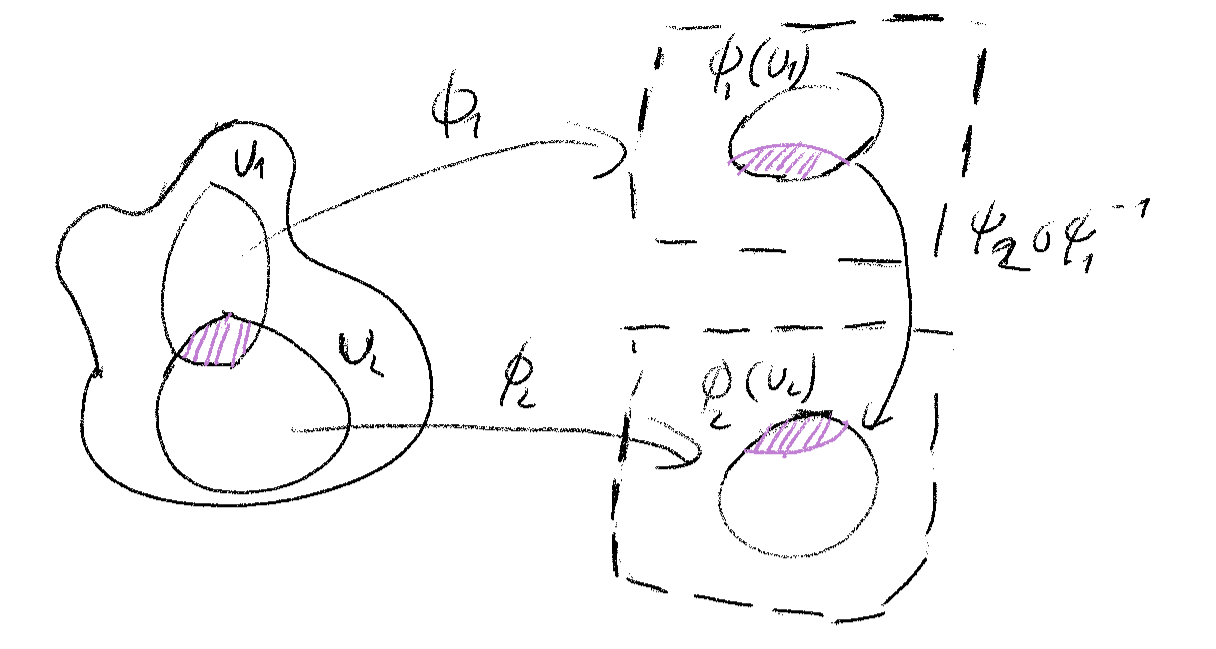
\includegraphics[width=.7\textwidth]{sketch_2_01.png}
        \caption{Sketch 2.01}
    \end{figure}
\end{definition*}

\begin{definition*}
    Let \(M\) be a topological manifold. An \dhighlight{(smooth) atlas} \(\cA\) of \(M\) is a collection of charts 
    \(\{U_\alpha,\phi_\alpha\}_{\alpha\in\cA}\) such that 
    \begin{itemize}
        \item the \(\{U_\alpha\}\) cover \(M\)
        \item the charts are pairwise smoothly compatible (i.e. for all \(\alpha,\beta\in\cA (U_\alpha,\phi_\alpha),(U_\beta,\phi_\beta)\) are smoothly compatible).
    \end{itemize}
\end{definition*}

\begin{definition*}
    We say that two atlases \(\cA,\cA'\) (on a fixed topological manifold) are \dhighlight{equivalent}, if their union 
    \(\cA\cup\cA'\) is still an atlas.
\end{definition*}

\dhighlight{Fact(Sheet 03):}
This defines an equivalence relation.

\begin{definition*}
    A \dhighlight{smooth manifold} \(M=(M,[\cA])\) consists of the following data:
    \begin{enumerate}
        \item[(i)] a topological manifolds \(M\)
        \item[(ii)] an equivalence class of smooth atlases 
    \end{enumerate}
\end{definition*}


\begin{remark}
    \begin{itemize}
        \item typically, we will designate smooth manifolds by a capital letter, e.g. \(M\). But we always mean \((M,[\cA])\).
              \dhighlight{Note} being a smooth manifolds is \dhighlight{extra} structure on a topological space, while being a topological manifold is a property
        \item Using Zorn's lemma, it can be shown that any atlas is contained in a \dhighlight{unique maximal atlas}. Uniqueness here does not use Zorn's lemma, only existence needs that! Equally well define a smooth manifold to 
              be a topological manifold and a maximal atlas.\marginnote{Typically we are given an atlas, since the maximal atlases have uncountably mani charts, which is why we work with equivalence classes, rather than maximal atlases}
        \item \(\forall 0\leq k\leq \infty\), we can define the notion of a \(C^k\)-atlas, simply by requiring that the transition functions are 
              \(C^k\) functions. This yields the definition of \(C^k\)-Manifolds. Two extreme cases: \(C^0\)-manifold (topological manifolds) and \(C^\infty\)-manifolds. Any \(k\geq 1\) is not more interesting than \(C^\infty\)!
    \end{itemize}
\end{remark}

\beginlecture{04}{18.10.2024}

\subsection{First examples of smooth manifolds}

\begin{example}[Example 1: The cannoical smooth manifold]
    \(\R^n,n\geq 0\) is \dhighlight{canonically} a smooth manifold. The \dhighlight{canonical atlas} is induced by 
    the topological chart \(U=\R^n,\phi:U\stackrel{\text{id}}{\to}\R^n\).
\end{example}

\begin{example}[Example 2: Another canonical smooth manifold]
    Let \(V\) be a finite dimensional real vector space . Then \(V\) is canonically a smooth manifold. Pick 
    a vector space basis \(\cB\). This basis induces a homeomorphism \(\phi_\cB: V\to\R^n\). If we had picked another basis \(\cB'\), then 
    then the transition map \(\phi_{\cB'}\circ \phi_\cB^{-1}\in\text{GL}(n,\R)\). Hence \(\phi_{\cB'}\circ \phi_\cB^{-1}\)
    is smooth.
\end{example}

\begin{example}[Example 3: Spheres]
    We have \(S_c^n\coloneqq\{(x_0,\dots,x_n)\in\R^{n+1}\mid \sum_{i=0}^n x_i^2=c^2\}\) for \(c>0\).
    Let \(\phi_i^{\pm}:\underbrace{U_i^{\pm}}_{\coloneqq \{(x_0,\dots,x_n)\in S_c^n\mid \pm x_i>0\}}\to B_c^n\).
    Then \(\phi_j^{\pm}\circ \left(\phi_{i}^{pm}\right)^{-1}(y_1,\dots,y_n)=\phi_j^\pm\left(y_1,\dots,\pm\sqrt{c^2-\sum y_i},\dots,y_n\right)\), where \((y_1,\dots,y_n)\in B_c^n\).
    \begin{align}
        =\begin{cases}
           (y_1,\dots,y_n) &i=j\\
            (y_1,\dots,\sqrt{c^2-\sum y_k},\dots,\hat{y_j},\dots,y_n) & j>i\\
            (y_1,\dots,\hat{y_{j+1}},\dots,\sqrt{c^2-\sum y_k},\dots,y_n) & j<i
        \end{cases}
    \end{align}
    We conclude \(\{U_{i}^\pm,\phi_i^\pm\}\) is a smooth atlas.
\end{example}

\begin{example}[Example 4: Level sets]
    Let \(\Phi:\R^{n+1}\to\R\) be a smooth function. Fix \(c\in\R\). Recall that the set \(\Phi^{-1}(c)=\{x\in\R^{n+1}\mid \Phi(x)=c\}\)
    is called a \dhighlight{level set} of value \(c\). \highlight{Suppose} that, \(\forall p\in \Phi^{-1}(c):D\underbrace{\Phi(p)}_{=(\partial_{x_0}\Phi(p),\dots,\partial_{x_n}\Phi(p))}\neq 0\).
    This means that \(\exists 0\leq i\leq n\) s.t. \(\partial_{x_i}\Phi(c)\neq0\). By the \dhighlight{implicit function theorem} (Lee, Theorem C.40, Course website),
    there exists a neighborhood \(U\) of \(p\) such that \(U\cap\Phi^{-1}(p)=\{(x_0,\dots,f(x_0,\dots,\hat{x_i},\dots,x_n),x_n)\}\).
    \begin{figure}[H]
        \centering
        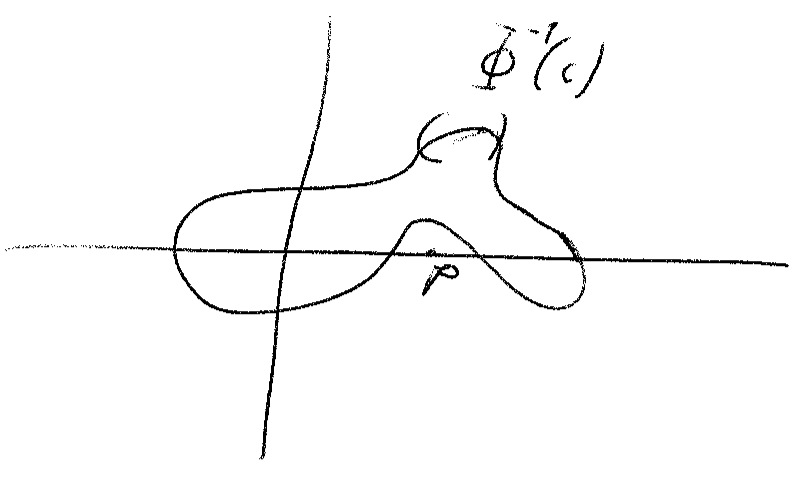
\includegraphics[width=.7\textwidth]{sketch_2_02.png}
        \caption{Sketch 2.02}
    \end{figure}

    Let \(M=\phi^{-1}(c)\). We define \(\hat{\pi_i}:\R^{n+1}\to\R^n,(x_0,\dots,x_n)\mapsto (x_0,\dots,\hat{x_i},\dots,x_n)\).
    \[\{(U,\hat{\pi_i})\mid U\subset M, \hat{\pi_i}\mid_U\text{ homeomorphism, } \partial_{x_i}\Phi\neq 0\text{ on } U\}\]

    Remains to check the formula:
    \[\hat{\pi_j}\circ \hat{\pi_i}^{-1}(y_1,\dots,y_n)=\begin{cases}
        (y_1,\dots,f,\dots,\hat{y_j},\dots,y_n)& j>i\\
        (y_1,\dots,\hat{y_{j+1}},\dots,f,\dots, y_n)& i<j\\
        (y_1,\dots,y_n) & i=j 
    \end{cases}\]
\end{example}

\begin{remark}
    The condition \(D\Phi\neq 0\) is very explicit! It is very easy to generate lots of manifolds. For example: \(\Phi(x)=\sum \lambda_i x_i^2\)
\end{remark}

\begin{example}[Example 5: Subset of smooth manifold] Let \(M\) be a smooth manifold. Then 
     \(U\subset M\) open, is also a smooth manifold. (Take charts of \(M\) and intersect / restrict each chart)
\end{example}

\begin{example}[Example 6: Product of manifolds] Let \(M,N\) be smooth manifolds. Then \(M\times N\) is also a 
    smooth manifolds. Take as charts \marginnote{This takes care of the torus!}
    \[\{(U\times V, (\phi,\psi))\mid (U,\phi),(V,\psi)\text{ charts of M,N respectively}\}\]
\end{example}

\begin{example}[Example 7: ]\marginnote{This is one to pay \dhighlight{attention} to!}
    Let's consider \(\R\). We define a chart \(\R\to\R,x\mapsto x^3\). Observe that 
    \[M=(U=\R,U\stackrel{\text{id}}{\to}\R)\]
    and 
    \[N=(U=\R,U\stackrel{x\mapsto x^3}{\to}\R)\]
    are smooth manifolds, which are different! Since the transition functions between them are not smooth:

    Indeed \(\text{id}\circ (x\mapsto x^3)^{-1}=(x\mapsto x^{\frac{1}{3}})\), which is not smooth!
\end{example}

\subsection{Smooth maps}

\begin{definition*}
    Let \(M\) be a smooth manifold. A map \(f:M\to\R^m\) is said to be \dhighlight{smooth}, if for all 
    \(p\in M\), there exists a chart \((U,\phi)\) containing \(p\), such that
    \[f\circ \phi^{-1}:\underbrace{\phi(U)}_{\subset\R^n}\to\R^m\] 
    is smooth. 
\end{definition*}

\begin{definition*}\marginnote{manifolds \(=\) smooth manifolds as always (unless otherwise stated)}
    Let \(M,N\) be manifolds. We say \(f:M\to N\) is \dhighlight{smooth} if, for all \(p\in M\) 
    there exists charts \((U,\phi)\) with \(p\in U\subset M\) and \((V,\psi)\) with \(V\subset N\) such that: 
    \begin{itemize}
        \item \(V\supset f(U)\)
        \item \(\psi\circ f\circ \phi^{-1}:\underbrace{\phi(U)}_{\subset\R^n}\to\R^m\) is smooth
    \end{itemize}
\end{definition*}

Reality check.

\begin{lemma}\label{lem:2.1}
    Smooth maps are continuous.
\end{lemma}

\begin{proof}
    Enough to show that \(\forall p\in M\), there exists a neighborhood of \(p\) on which \(f:M\to N\) is 
    continuous, for \(f\) smooth. By definition \(\exists (U,\phi),p\in U,(V,\psi),V\subset N\) s.t. 
    \(\psi \circ f\circ \phi^{-1}:\phi(U)\to\R^m\) smooth.

    Observe \(f=\psi^{-1}\circ (\psi \circ f\circ \phi^{-1})\circ \phi\) on \(U\).
\end{proof}

\begin{lemma}\label{lem:2.2}
    \(f:M\to N\) is smooth if and only if each \(p\in M\) has a neighborhood \(U\) such that \(f\mid_U\) is smooth.
\end{lemma}

\begin{proof}
    Sheet 03.
\end{proof}

\begin{lemma}[Properties of smooth maps]
    \begin{enumerate}
        \item[(i)] Any constant map \(c:M\to N\) is smooth\footnote{Since it sends \(M\) to a point in \(N\)}
        \item[(ii)] The identity map \(\text{id}:M\to M\) is smooth 
        \item[(iii)] If \(U \circ M\) open, then the inclusion \(i:U\hookrightarrow  M\) is smooth
        \item[(iv)] Compositions of smooth functions are smooth
    \end{enumerate}
\end{lemma}

\begin{proof}
    Sheet 03.
\end{proof}

\begin{definition*}\marginnote{In particular, diffeomorphisms are homeomorphism!}
    Let \(M,N\) be manifolds. A \dhighlight{diffeomorphism} \(f:M\to N\) is a smooth 
    map, which is bijective and admits a smooth inverse.
\end{definition*}

\begin{example}
    \(f:\R\to\R,x\mapsto x+3\) is a diffeomorphism with inverse \(x\mapsto x-3\).  
\end{example}

\begin{example}
    Let \(A\in\text{GL}(n,\R)\). Define a map \[f_A:\R^n\to\R^n,x\mapsto Ax.\]
    This is a diffeomorphism (smooth, since linear) with inverse \(f_A^{-1}=f_{A^{-1}}\).  
\end{example}

\begin{example}
    Let \(S_c^n\coloneqq \{(x_0,\dots,x_n)\mid \sum_{i=0}^n x_i^2=c^2\}\subset\R^{n+1}\). Given 
    \(d>c>0\), we define a diffeomorphism. 
    \[S_c^n\to S_d^n, (x_0,\dots,x_n)\mapsto \frac{d}{c}(x_0,\dots,x_n).\]
\end{example}

\begin{example}
    \(M=(\R,\text{id}),N=(\R,x\mapsto x^3)\). The map \(M\to N, x\mapsto x^{\frac{1}{3}}\)
    is a diffeomorphism. Indeed, 
    \begin{align*}
        (x\mapsto x^3)\circ (x\mapsto x^{\frac{1}{3}}) \circ\text{id}^{-1}=\text{id}
    \end{align*}
\end{example}

\subsection{The category of smooth manifolds}

\begin{definition*}
    Let \(\text{Man}^\infty\) be the category of smooth manifolds. The objects are the smooth manifolds. 
    The morphisms are the smooth maps.
\end{definition*}

\dhighlight{Exercise}: \(M,N\) objects in \(\text{Man}^\infty\) are isomorphic if and only if they are diffeomorphic.

Observe that there is a forgetful functor: \(\maninf\to\man0\) by \( (M,[\cA])\to M\) and \(f:M\to N\mapsto f\).

In general:\begin{itemize}
    \item not full 
    \item not essentially surjective
\end{itemize}

\begin{remark}[Hierarchy of categories]
    \begin{itemize}
        \item for \(k=0,\dots,\infty\), we can consider the category \(\mank\) with objects \(C^k\)-Manifolds, and morphisms \(C^k\)-maps. 
              for \(k\leq l\) there is a forgetful functor \(\text{Man}^l\to\mank\)
        \item if \(k\geq 1\),then the forgetful functor \(\maninf\to\mank\) is essentially surjective. This is different from the \(C^0\) case. For this reason, we mainly focus on \(\man0,\maninf\). This is a theorem by Whitney
        \item there are other interesting categories: \(\text{Man}^{\text{Real-analytic}},\text{Man}^{\text{Cplx-analytic}},\dots\), which both come with a forgetful functor to \(\maninf\)
    \end{itemize}
\end{remark}

\begin{remark}[Classification of manifolds (not examinable)]
    \begin{itemize}
        \item all topological manifolds of dimension \(\leq 3\) admit a unique smooth structure
        \item \(S^7\), as a topological manifold, admits 15 pairwise non-diffeomorphic smooth structures. These are called \dhighlight{exotic spheres}. They also exist 
            in higher dimensions (Milan-Kervaire?)
        \item \(\R^4\) admits uncountably many pairwise non-diffeomorphic smooth structures (Taubes~1980s)
        \item Open problem(\dhighlight{Smooth 4 dimensional Poincaré conjecture}): Prove or disprove: any smooth 
              4-manifold, which is homeomorphic to \(S^4\) is diffeomorphic to \(S^4\). Most experts believe this is false!  
    \end{itemize}
\end{remark}

\beginlecture{05}{22.10.2024}

\subsection{Smooth manifolds with boundary} % TODO: Wrong number?

\begin{definition*}
    A function \(f:\bH^n\supset U \to \R^k\) is \dhighlight{smooth} if every \(p\in U\)
    admits an open neighborhood \(p\in U_p\subset\R^n\) on which \(f\) extends to a smooth function. (i.e. there exists \(\tilde{f}_p:U_p\to\R^k,\tilde{f}_p\) smooth and \(\tilde{f}_p\mid_{\bH^n\cap U}=f\))
\end{definition*}

\begin{figure}[H]
    \centering
    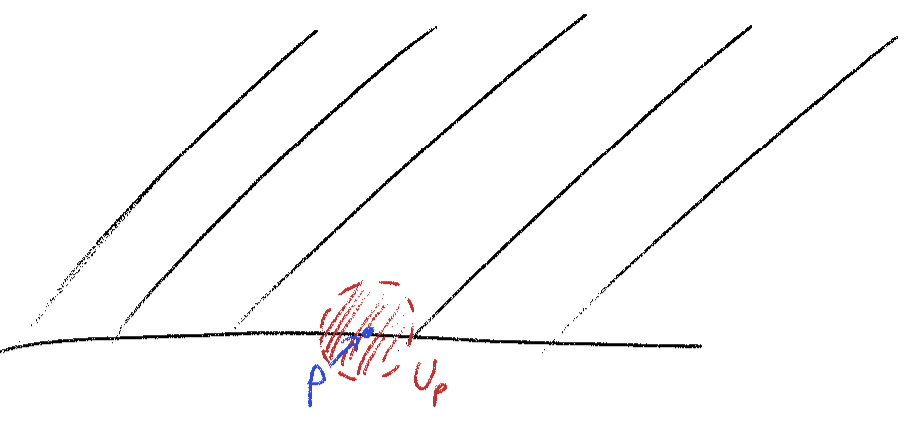
\includegraphics[width=.7\textwidth]{sketch_2_03.png}
    \caption{Sketch 2.03}
\end{figure}

\begin{example}
    \(n=1,\bH^1=[0,\infty), f(x)=x^2\)
\end{example}
\begin{example}[Non-Example]
    \(n=1,\bH^1=[0,\infty), f(x)=\sqrt{x}\) has no smooth extension to \(0\), since the derivative goes to \(\infty\).
\end{example}

Give a topological manifold with boundary, we can define unproblematically the notions of 
\begin{itemize}
    \item smoothly compatible charts: \((U,\phi):M\to\bH^n\), \(\phi_\alpha\circ \phi_\beta^{-1}:\phi_\beta(U_\alpha\cap u_\beta)\to\bH^n\)
    \item smooth atlases
\end{itemize}

\begin{definition*}
    A smooth manifold with boundary \(M=(M,[\cA])\) is the data of 
    \begin{itemize}
        \item a topological manifold with boundary 
        \item an equivalence class of atlases 
    \end{itemize}    
\end{definition*}

\begin{remark}\marginnote{Similarly we cna generalise even more to manifolds with corners ...}
    Every smooth manifold is a smooth manifold with boundary. This is an enlargement of 
    \(\maninf\).
\end{remark}

\section{Partitions of unity}\marginnote{This section is technical, but also very important!}

\subsection{Preparatory lemmas}

\begin{lemma}\label{lem:2.4}
    The function \(f:\R\to\R,\)
    \[f(t)=\begin{cases}
        e^{-\frac{1}{t}} & t>0\\
        0 & t\leq 0
    \end{cases}\]
    is smooth.
\end{lemma}

\begin{figure}[H]
    \centering
    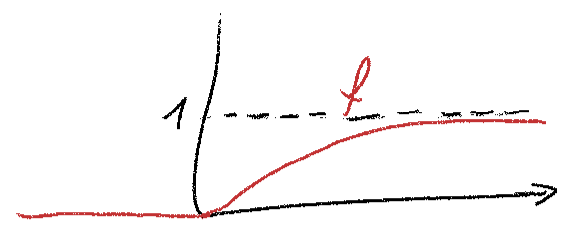
\includegraphics[width=.7\textwidth]{sketch_2_04.png}
    \caption{Sketch 2.04}
\end{figure}

\begin{proof}
    It is enough to proof, that \(f\) has well defined derivatives of all orders, since \(f\) is a function on \(\R\).

    \(f^0=f\), for  \(k\geq 1\), assume \begin{enumerate}
        \item \(f^{(k-1)}\) exists
        \item \(f^{(k-1)}\mid_{(-\infty,0]}=0\) 
        \item \(f^{(k-1)}\mid_{(-\infty,0]}(t)=P_{k-1}(\frac{1}{t})e^{-\frac{1}{t}}\) for some polynomial \(P_{(k-1)}\).
    \end{enumerate}
    Clearly this holds for \(k=1\). 
    
    We have \begin{align*}
        \lim_{t\to0^+}\frac{f^{(k-1)}(t)-f^{(k-1)}(0)}{t}&=\lim_{t\to 0^+}\frac{f^{(k-1)}(t)}{t}\\
        &=\lim_{t\to 0^+}P_{(k-1)}(\frac{1}{t})\frac{1}{t}e^{-\frac{1}{t}}\\
        &= \lim_{x\to\infty} P_{(k-1)}(x)\cdot x\cdot e^{-x}=0
    \end{align*}
    Therefore \(f^{(k-1)}\) is differentiable at the origin, the derivative \(f^{(k-1)'}(0)=0\).
    and \(f^{(k-1)}\mid_{(-\infty,0]}=0\). Therefore \(f^{(k-1)}\) is differentiable.
    Therefore we only have to check 3., which only takes place on \(\R_+\)! 

    Finally \(f^{(k-1)}\mid_{(0,\infty)}(t)=P_{(k-1)}(\frac{1}{t})e^{-\frac{1}{t}}\implies P_{(k-1)}'(\frac{1}{t})\left(\frac{-1}{t^2}e^{-\frac{1}{t}}+P_{(k-1)}(\frac{1}{t})e^{-\frac{1}{t}}\right)\eqqcolon P_{(k)}(\frac{1}{t})e^{-\frac{1}{t}}\).
\end{proof}

\begin{lemma}\label{lem:2.5}
   Fix real numbers \(r_1<r_2\). Then there exists a smooth function \(h:\R\to\R\) such that 
   \begin{enumerate}
    \item \(h\equiv 1\) on\((-\infty,r_1]\)
    \item\(0<h<1\) on \(r_1,r_2\)
    \item \(h\equiv 0\) on \([r_2,\infty)\)
    \end{enumerate}
\end{lemma}

\begin{proof}
    \(h(t)\coloneqq \frac{f(s_2-t)}{f(s_2-t)+f(t-s_1)}\), since the denominator never goes to \(0\).
\end{proof}

\begin{lemma}[Existence of \dhighlight{cutoff functions}]\label{lem:2.6}
    Given \(0<r_1<r_2\), there exists a smooth function \(H:\R^n\to\R\) such that 
    \begin{enumerate}
        \item \(H\equiv 1\) on \(\overline{B_{r_1}}\)
        \item \(0<H<1\) on \(B_{r_2}\setminus \overline{B_{r_1}}\)
        \item \(H\equiv 0\) on \(\R^n\setminus B_{r_2}\)
    \end{enumerate}
\end{lemma}

\begin{proof}
    Set \(H(x)\coloneqq h(|x|)\), where \(h\) is defined as in lemma \ref{lem:2.5}. (Recall: \(|x|\coloneqq \sqrt{x_1^2+\dots+x_n^2}\)).
    Then \(H\) is smooth, since it is a composition of smooth functions on \(\R^n\setminus \overline{B_{r_1}}\) and constant on \(\overline{B_{r_1}}\).
\end{proof}

\subsection{Partitions of unity}

\begin{definition*}
    Given a topological space \(X\) and a function \(f:X\to\R\), the \dhighlight{support} of \(f\) is the set 
    \[\supp(f)\coloneqq\overline{ \{x\in X\mid f(x)\neq 0\}}\subset X\]
\end{definition*}

\begin{example}
    If \(f:\R\to\R\) has the form \(f(x)=a_0+a_1x+\dots,a_nx^n\implies \supp(f)=\R\).
    In fact, by Taylor's theorem, if \(f\) analytic, then \(\supp(f)\) either \(\R\) or \(\emptyset\).
    In contrast, the function \(h:\R\to\R\) defined in lemma \ref{lem:2.5} has support \((-\infty,r_2]\subsetneqq\R\).
\end{example}

\begin{definition*}
    Let \(M\) be a smooth manifold. Let \(\{U_\alpha\}_{\alpha\in \cA}\) be an open cover. 
    A \dhighlight{partition of unity subordinate to the cover} is the data of a collection of smooth functions \(\{\psi_\alpha\}_{\alpha\in\cA},\psi_\alpha:M\to\R\)
    such that 
    \begin{enumerate}
        \item[(1)] \(0<\psi_\alpha<1\)
        \item[(2)] \(\supp(\psi_\alpha)\subset U_\alpha\)
        \item[(3)] \(\{\supp(\psi_\alpha)\}_{\alpha\in\cA}\) is locally finite 
        \item[(4)] \(\sum_{\alpha\in\cA} \psi_\alpha\equiv 1\)    
    \end{enumerate}
\end{definition*}

\begin{remark}
    There is an analogous notion in the category Top,\(\man0,\mank\), etc.,\dots
\end{remark}

\begin{example}
    \(M=\R\), \(U_1=(-\infty,r_2+1),U_2=(r_1-1,\infty)\), where \(r_1<r_2\) as in lemma \ref{lem:2.5}.
    Similarly let \(h\) as in lemma \ref{lem:2.5}. and set \(\psi_1=h,\psi_2=1-h\)
    \begin{figure}[H]
        \centering
        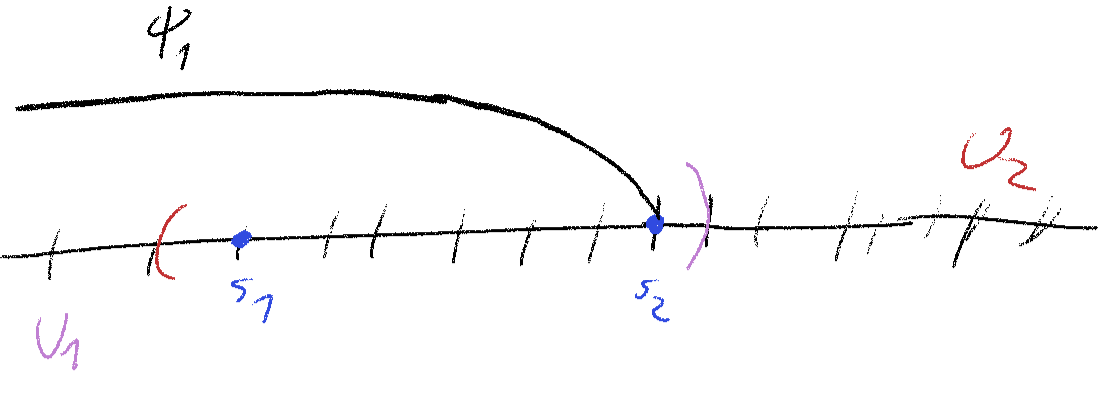
\includegraphics[width=.7\textwidth]{sketch_2_05.png}
        \caption{Sketch 2.05}
    \end{figure}
\end{example}

\begin{theorem}[Existence of partitions of unity]\label{thm:2.7}
    Let \(M\) be a smooth manifold. Let \(\{U_{\alpha}\}_{\alpha\in\cA}\) be an open cover. 
    Then there exists a partition of unity subordinate to this cover. 
\end{theorem}

\begin{remark}
    The same theorem works in Top, \(\man0,\mank\). It will not work in \(\text{Man}^{\text{Analytic}},\text{Man}^{\text{Cplx-Analytic}},\) Varieties \(/\C\).
\end{remark}

\begin{proof} % TODO: correct step 01
    \dhighlight{Step 1: Construction of the \(V_i\)} An open supset \(U\subset M\) is called a \dhighlight{regular coordinate ball} if there 
    exists \(\overline{U}\subset\tilde{U},(\tilde{U},\tilde{\phi})\) a chart such that 
    \(\tilde{\phi}(U)=B_{r_1},\tilde{\phi}(\tilde{U})=B_{r_2}\). 
    \begin{figure}[H]
        \centering
        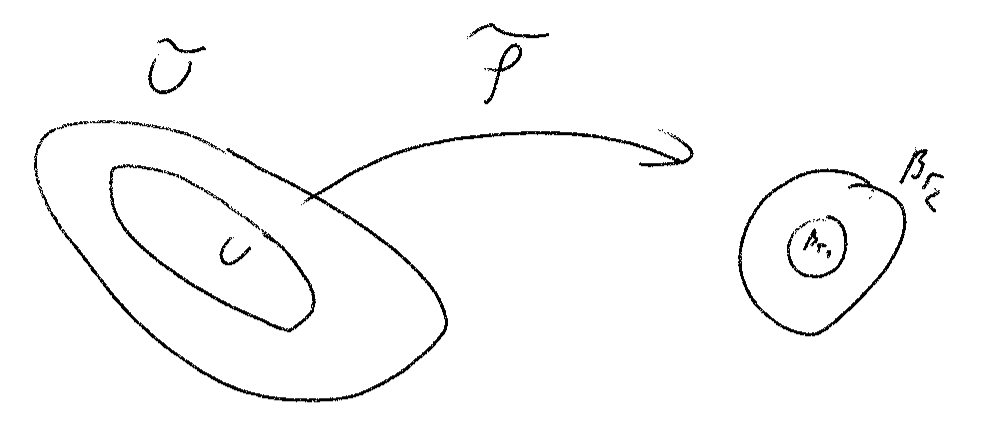
\includegraphics[width=.7\textwidth]{sketch_2_06.png}
        \caption{Sketch 2.06}
    \end{figure}
    By lemma \ref{lem:1.6} \(M\) admits an exhaustion by compact sets. By lemma \ref{lem:1.7}, given 
    any basis, any open cover, one can find a locally finite, countable basis refinement of this cover by basis elements.

    Claim: \(\{\text{regular coordinate balls whose closure is contained in some }U_\alpha\}\) basis of \(M\) \marginnote{The claim is easy to verify}

    These tree points imply that \(\{U_\alpha\}_{\alpha\in\cA}\) admits a countable, locally finite refinement by regular coordinate balls \(\{V_i\}_{i\in I}\).

    By sheet 2, exercise 1 (a) \(\{\overline{V_i}\}\) is still locally finite.

    \dhighlight{Step 2: Construction of the \(f_i\)} For each \(V_i\exists V_i\supset \tilde{V_i},\tilde{\phi_i}:\tilde{V_i}\to \R^n\) such that 
    \(\tilde{\psi_i}(V_i)=B_{r_1^i},\tilde{\psi_i}(\tilde{V_i})=B_{r_2^i}\) with \(0<r_1^i<r_2^i\), \(\tilde{V_i}\subset U_\alpha\) for some \(\alpha\).
    Using lemma \ref{lem:2.6}, let \(H_i:\R^n\to \R\) be a cutoff function, i.e. \(H_i\mid_{{B_{r_1}}}>0,H=0\) on \(\R\setminus B_{r_1^i}\).
    \marginnote{Finging \(\tilde{V}_i\) s.t. \(\tilde{V}_i\subset U_\alpha\) is the reason we considered regular coordinate balls whose \dhighlight{closure is contained} in some \(U_\alpha\)}
    Let us set \(f_i:M\to\R, f_i=\begin{cases}
        H_i\circ \tilde{\phi_i} & \text{ on } \tilde{V_i}\\
        0 & M\setminus \overline{{V_i}}
    \end{cases}\)

    \dhighlight{Step 3: Construction of the \(g_i\)} Let us set \(f=\sum_{i\in I} f_i\). This is well defined by local finiteness of the \(\overline{V_i}\) Note also that \(f>0\)..
    We set \(g_i=f_i/f\). Then clearly we have \(0\leq g_i\leq 1, \sum_{i\in I} g_i\equiv 1\)

    \dhighlight{Step 4: Reindexing and conformation} Since \(\tilde{V_i}\subset U_\alpha\), for some \(\alpha\), we can choose for each \(i\in I, \alpha(i)\in \cA\) s.t. \(V_i\in U_{\alpha(i)}\).
    Let us set \marginnote{Here the empty sum is \(0\)}\[\psi_{\alpha}\coloneqq \sum_{i\mid \alpha=\alpha(i)}g_i\]
    Observe for \dhighlight{(2)}: \[\supp(\psi_\alpha)=\overline{\bigcup_{\alpha(i)=\alpha} V_i}\stackrel{\text{Exercise 2.1}}{=}\bigcup_{\alpha(i)\alpha}\overline{V_i}\subset U_\alpha\]
    We still have \(0\leq \psi_\alpha\leq 1\), which is \dhighlight{(1)}
    
    and 
    \(\supp(\psi_\alpha)\) are locally finite: for each \(op\in M\), since \(\{\overline{V_i}\}\) locally finite,
    there exists a neighborhood \(U_p\) of \(p\)  which only intersects finitely many of the \(\{\overline{V_i}\}\), call 
    them \(V_1,\dots,V_k\). Then the only \(\psi_\alpha\) which have a chance of being non-zero must satisfy \(\alpha\in\{\alpha(1),\dots,\alpha(k)\}\) (this is \dhighlight{(3)}).

    Lastly \[\sum_{\alpha\in\cA}\psi_\alpha=\sum_{\alpha}\left(\sum_{i: \alpha=\alpha(i)} g_i\right)=\sum_{i\in I} g_i\equiv 1,\]
    which confirms \dhighlight{(4)}.

\end{proof}

\beginlecture{06}{25.10.2024}

\subsection{Applications of partitions of unity}

\begin{definition*}
    Let \(X\) be a topological space. Let \(A\subset X\) be closed, \(U\subset X\), \(A\subset U\) be open. 
    A \dhighlight{bump function for \(A\)} supported in \(U\) is a function \[\phi:X\to\R\]
    such that \(\psi\mid_A \equiv1, \supp(\phi)\subset U\). 
\end{definition*}

\begin{figure}[H]
    \centering
    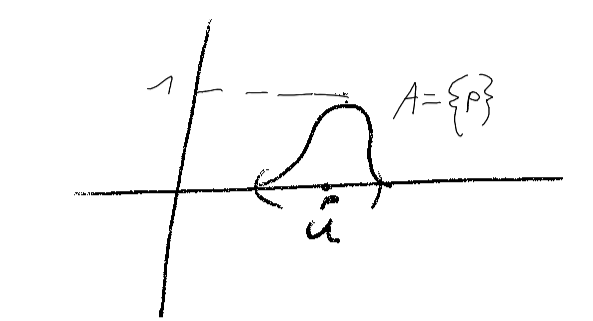
\includegraphics[width=.7\textwidth]{sketch_2_07.png}
    \caption{Sketch 2.07}
\end{figure}

\begin{proposition}\label{prop:2.8}
    Let \(M\) be a smooth manifold. Fix \(A\subset M\) closed, \(U\subset M,A\subset U\subset M\) open.
    Then there exists a smooth bump function for \(A\) supported in \(U\)
\end{proposition}

\begin{proof}
    Let \(V=M\setminus A\). Then \(\{U,V\}\) is a covering and  by theorem \ref{thm:2.7}, there exist 
    \(\{\Psi_U,\Psi_V\}\) partitions of unity subordinate to this cover. Now \(\Psi_U\) does the job.
\end{proof}

\begin{definition*}
    Let \(M,N\) be smooth manifolds. Let \(A\subset M\) be closed. We say that \(f:A\to N\) is smooth 
    if it admits a smooth extension in a neighborhood of each point \(p\in A\). \marginnote{I.e. for any \(p\in A\) there exists \(U_p\ni p,\) a smooth function \(\tilde{f}_p:U_p\to N\) s.t. \(\tilde{f}_p\mid_{U_p\cap A} = f\mid_{U_p\cap A}\)}
\end{definition*}

\begin{proposition}\label{prop:2.9}
    Let \(M\) be a smooth manifold. Let \(A\subset M\) be closed and \(f:A\to\R^k, k\geq 0\) be smooth.
    Then for any open \(U \subset M, A\subset U\), there exists \(\tilde{f}:M\to\R^k\), such that \(\tilde{f}\mid_{A}=f\) and \(\supp(\tilde{f})\subset U\)
\end{proposition}

\begin{remark}
    This would be \dhighlight{false} if we replaced \(\R^k\) by an arbitrary smooth manifold \(N\). E.g. 
    take \(\R^2\hookleftarrow A=S^1\stackrel{f=\text{id}}{\to}S^1\)
\end{remark}

\begin{proof} % TODO: Fix restrictions
    For each \(p\in A\), choose a neighborhood \(p\in W_p\subset U\)\marginnote{We maybe need \(\overline{W_p}\subset U\)? Prob. not?}, \(\tilde{f}_p:W_p\to\R^k\) smooth 
    extension of \(f\mid_{A\cap W_p}\). Then observe that \(\{W_p\}_{p\in A}\cup (M-A)\) forms an open cover of \(M\).
    \(\{\psi_p\}_{p\in A}\cup \psi_0\) be a partition of unity subordinate to the cover. Now we set 
    \(\tilde{f}=\sum_{p\in A}\psi_p \tilde{f}_p\). By local finiteness \(\tilde{f}\) is smooth. Also 
    \begin{align*}
        \tilde{f}\mid_A&=\sum_{p\in A} \psi_p\mid_A \underbrace{\tilde{f_p}\mid_A}_{=f}\\
        &=f\sum_{p\in A} \psi_p\mid_A = f\mid_A \cdot 1 = f\mid_A .\qedhere
    \end{align*}
\end{proof}

\begin{definition*}
    Let \(X\) be a topological space. An \dhighlight{exhaustion function} \(f:X\to\R\) is a 
    continuous function such that \(\forall C\in \R,f^{-1}(-\infty,c]\) is compact. \marginnote{If \(X\) is compact every \(f\) is an exhaustion function \dots}
\end{definition*}

\begin{example}
    \(X=\R,f:\R\to\R,x\stackrel{f}{\mapsto} x^2\)
\end{example}

\begin{example}[NON-EXAMPLE]
    \(X=\R,f(x)=x\)
\end{example}

\begin{proposition}\label{prop:2.10}
    Every smooth manifold admits a smooth exhaustion function.
\end{proposition}

\begin{proof}
    Pick a countable partition of unity \(\{U_i\}_{i\in N_+}\) by open subsets having compact closure\footnote{Like in the proof of \ref{thm:2.7}}.
    Let \(\{\Psi_i\}_{i\in\N_+}\) be a subordinate partition of unity. Let \(f\coloneqq \sum_{i\in\N_+}i\psi_i\).
    
    Observe that for any \(c\in\R\), \(c<N\in \N\) that \[f^{-1}(-\infty,c]\subset f^{-1}(-\infty,c]\subset \bigcup_{i=1}^N \overline{U_i}\]

    Why \(f^{-1}(-\infty,c]\subset\bigcup_{i=1}^N \overline{U_i}\)? Let \(q\not\in \bigcup_{i=1}^N \overline{U_i}\).
    Then \begin{align*}
        f(q)&=  \underbrace{\sum_{i=1}^{N} i \psi_i(q)}_{=0} + \sum_{i=N+1}^\infty i\psi_i(q)\\
        & \geq (N+1)\sum_{i=N+1}^\infty\psi_i(q) = (N+1)\underbrace{\sum_{i=1}^\infty \psi_i(q)}_{=1}\\
        &=N+1 
    \end{align*} 
\end{proof}

 \begin{proposition}\label{prop:2.11}
    Let \(M\) be a smooth manifold. Let \(A\subset M\) be a closed subset. Then 
    there exists a smooth function \[f:M\to\R,f^{-1}(0)=A\]
    \marginnote{In fact, the prove shows one can assume \(f\geq 0\)}
 \end{proposition}

 E.g. take \(M=\R,A=\) Cantor set, shows that this is non-trivial.

 \begin{proof}
    Assume \(M=\R^n\) (general case: Sheet 04).

    Choose a countable cover of \(\R^n\setminus A\) by balls \(\{B_{r_i}(x_i)\}_{i=1}^\infty\) with \(r_i<1\).
    By Lemma \ref{lem:2.6} there exists a cutoff function \[H:\R^n\to \R\]
    s.t. \(H\equiv 1\) on \(\overline{B_{\frac{1}{2}}(0)}\) and \(0<H<1\) on \(B_1(0)\setminus \overline{B_{\frac{1}{2}}(0)}\)
    and \(H\equiv 0\) on \(R^n\setminus B_1(0)\). For each \(i\geq 1\) let \(C_i\gg 1\) be large enough so that 
    \[C_i>\sup \{\partial^\alpha_x H \mid \alpha=\overbrace{(\alpha_1,\dots,\alpha_n)}^{\in \N^n},|\alpha|\leq i\}\]  

    Let \[f\coloneqq \sum_{i=1}^\infty \frac{r_i^i}{2^i c_i}H\left(\frac{x-x_i}{r_i}\right).\]
    We need to argue that \(f\) is smooth. Observe that, since \(r_i<1\) \(\frac{r_i}{2^ic_i}H\left(\frac{x-x_i}{r_i}\right)\leq \frac{1}{2^i}\)
    It follows from Analysis 2 that \(f\) is continuous. To prove that \(f\) is smooth assume for \(k\geq 1\)  
    that all partial of order \(k<1\) exist and are continuous. If \(|\alpha|=k\), then \begin{align*}
        \partial^\alpha\frac{r_i^i}{2^iC_i} H\left(\frac{x-x_i}{r_i}\right)=\frac{r_i^{i-k}}{2^iC_i}\partial^\alpha H \left(\frac{x-x_i}{r_i}\right)
    \end{align*}
    If \(i>k\), then 
    \begin{align*}
        \left\vert \frac{r_i^{i-k}}{2^iC_i} \partial^\alpha  H \left(\frac{x-x_i}{r_i}\right)\right\vert<\frac{1}{2^i}
    \end{align*}
    Again follows by Analysis 2 that \(\partial^\alpha f\) exists and equals \(\sum\partial^\alpha \left(\frac{r_i^i}{2^iC_i}H\left(\frac{x-x_i}{r_i}\right) \right)\).
\end{proof}

